\documentclass{article}
\usepackage[utf8]{inputenc}
\usepackage[english]{babel}
\usepackage{graphicx}
\usepackage{amsthm}

\DeclareGraphicsExtensions{.pdf,.ps,.png,.jpg}

\newcounter{results}

\newtheorem{theorem}{Theorem}[section]
\newtheorem{lemma}[theorem]{Lemma}
\newtheorem{corollary}{Corollary}[theorem]

\author{
  McCaffrey, Caitie\\
  \texttt{Sporty Tights, Inc}
  \and
  Kingsbury, Kyle\\
  \texttt{The SF Eagle}
  \and
  Narula, Neha\\
  \texttt{That's DOCTOR Narula to you!}
}

\title{Distributed Sagas}

\begin{document}

\maketitle

\section{Introduction}

The saga paper outlines a technique for long-lived transactions which provide
atomicity and durability without isolation (what about consistency? Preserved
outside saga scope, not within, right?). In this work, we generalize sagas to
a distributed system, where processes communicate via an asynchronous network,
and discover new constraints on saga sub-transactions.

We are especially interested in the problem of writing sagas which interact with
\textit{third-party services}, where we control the Saga Execution Coordinator
(SEC) and its storage, but not the downstream Transaction Execution
Coordinators (TECs) themselves. Communication between the SEC and TEC(s) takes
place over an asynchronous network (e.g. TCP) which is allowed to drop, delay,
or reorder messages, but not to duplicate them.

We assume a high-availability SEC service running on multiple nodes for
fault-tolerance, where multiple SECs may run concurrently. They coordinate
their actions through a linearizable data store, which ensures saga
transactions proceed sequentially.

\section{The Saga Execution Coordinator}

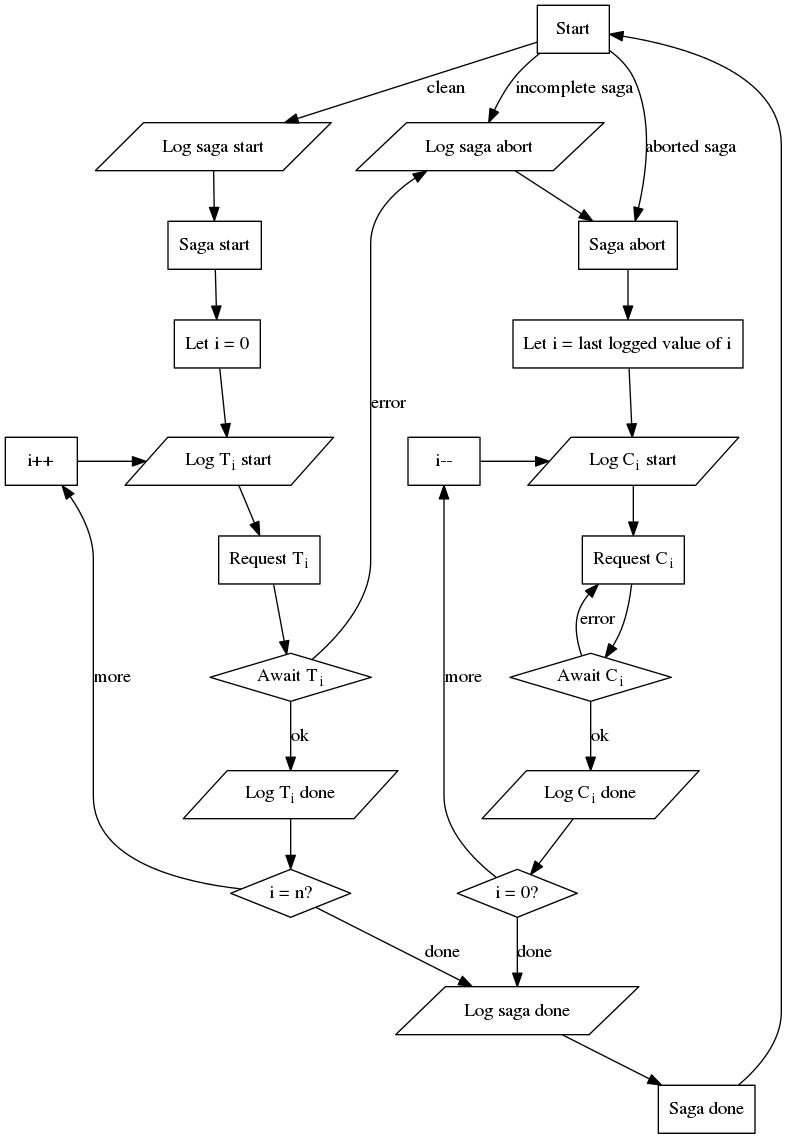
\includegraphics[width=\linewidth]{flow}




\section{Both Rollback and Roll-forward}

\begin{lemma}[]
\label{t_contiguous}
If $T_i$ is received by a TEC, then $T_0, T_1, ... T_{i-1}$ have already been
acknowledged by a TEC, where $0 < i \le n$.
\end{lemma}

\begin{proof}

In order for $T_i$ to be received by a TEC, it must have been requested by an
SEC. In a roll-forward SEC, this could be a retry of a failed attempt to
execute $T_i$, but regardless of whether the SEC is roll-back or roll-forward,
entering that part of the algorithm requires the SEC to journal its intent to
start $T_i$.

There are only two paths to that journaling operation. The first case, $i = 0$,
falls outside our constraint $0 < i \le n$. Therefore the SEC \textit{must}
have taken the other path: incrementing $i$ before beginning a new transaction.

That path depends on $i - 1 \ne n$ being false, which holds since we are
considering $i \le n$. That in turn depends on journaling $T_{i-1}$'s
completion, which depends on a successful response from a TEC for $T_{i-1}$.
Therefore some TEC acknowledged $T_i$. That in turn requires that TEC to have
received $T_i$.

So, the receipt of $T_i$ implies both the receipt and acknowledgement of
$T_{i-1}$. By induction, receiving $T_i$ implies \textit{all} transactions
$T_0, T_1, ... T_{i-1}$ have been acknowledged.

\end{proof}


\begin{corollary}
\label{t_zero_first}
The first transaction to be received and acknowledged is $T_0$.
\end{corollary}

\begin{proof}
Assume the first transaction to be processed is not $T_0$, but rather, some
$T_i \mid 0 < i \le n$. By \ref{t_contiguous}, $T_{i-1}$ must have been
received and acknowledged by a TEC already. $T_i$ is therefore \textit{not} the
first transaction: a contradiction.
\end{proof}



\section{Rollback}

\begin{lemma}
\label{t_at_most_once}
Transactions are requested and received at most once.
\end{lemma}

\begin{proof}
In order for an SEC to request a transaction $T_i$, it has to record its intent
to execute $T_i$ in shared SEC storage. Since that storage is linearizable, any
other SEC recording an intent to execute $T_i$ would be visible to the
requesting SEC.

\begin{description}
  \item[Case 1] Another SEC has already recorded its intent to request $T_i$.
The given SEC chooses to crash instead of requesting $T_i$.
  \item[Case 2] No other SEC has recorded its intent to request $T_i$. The
given SEC requests $T_i$ once.
\end{description}

In both cases, $T_i$ is requested at most once, across all SECs, depending on
whether or not the successfully-recording SEC crashes before making its
request.

Because the network does not duplicate requests, the number of times $T_i$ can
arrive at a TEC is less than or equal to the number of requests any SEC makes
for $T_i$. Since that number is at most one, $T_i$ is received at most once.
\end{proof}


\begin{lemma}
\label{t_sequential}
Transactions are seen by TECs in sequential order: $T_0, T_1, \ldots, T_j$,
where $0 \le j \le n$.
\end{lemma}

\begin{proof}

Let the $i^{th}$ transaction seen be $T_j$. We wish to show $i = j$.

How many transactions appear prior to $T_j$? By \ref{t_contiguous}, at least
$j$ transactions ($T_0, \ldots T_{j-1}$) must have already executed prior to
$T_j$. This implies $j <= i$.

Assume $j < i$. Then there must be some transaction $T_k$, prior to $T_j$, in
addition to the minimum required $T_0, \ldots, T_{j-1}$. \ref{t_at_most_once}
rules out $T_k$ being a duplicate of any other transaction, so $j < k$.
However, this implies $T_k$ appears with fewer than $i$ transactions before it.


\end{proof}



\end{document}
